\chapter{Trying to Verify checkTransaction}
\label{chap:verify_check}

This chapter describes some parts of Bitcoin-S needed to verify our property.
We are going to create a transaction and show you the relevant parts of checkTransaction, where transactions are checked against some properties.
Then we see some troubles occurred during this work.
In the end you will see how we fixed a bug in Bitcoin-S.


\section{Creation of a Transaction}

Some of the code in this section are copied or modified parts of Bitcoin-S-Core transaction builder example.\cite{BitcoinSCore:txbuilderexample}
Bitcoin-S-Core has a bitcoin transaction builder class with the following signature:
\begin{lstlisting}[language=scala]
  BitcoinTxBuilder(
    destinations: Seq[TransactionOutput], // where we send money
    utxos: BitcoinTxBuilder.UTXOMap,      // unspent transaction outputs
    feeRate: FeeUnit,                     // fee rate per byte
    changeSPK: ScriptPubKey,              // public key
    network: BitcoinNetwork               // bitcoin network information
  ): Future[BitcoinTxBuilder]             // sign TxBuilder to get tx
\end{lstlisting}

Here is how those parameters are generated.

First, we need a some bitcoins/satoshis.
Thus, we create a transaction with one single output.
This transaction can also be parsed from the real bitcoin network but to show the progression we create one.
\begin{lstlisting}[language=scala]
  val privKey = ECPrivateKey.freshPrivateKey
  val creditingSPK = P2PKHScriptPubKey(pubKey = privKey.publicKey)

  val amount = Satoshis(Int64(10000))

  val utxo = TransactionOutput(currencyUnit = amount, scriptPubKey = creditingSPK)

  val prevTx = BaseTransaction(
    version = Int32.one,
    inputs = List.empty,
    outputs = List(utxo),
    lockTime = UInt32.zero
  )
\end{lstlisting}

On line one and two we are creating a new keypair to sign the next transaction and have a scriptPubKey where the bitcoins are.
Line four specifies the amount of satoshis we are having in the transaction.
Then we create the actual transaction from line 6 to 13.

Now that we have some bitcoins, we create the new transaction to spend them.

First, we need some out points.
This are pointers to previous transactions' outputs.
We use the index zero, because the previous transaction has only one output that becomes the first index zero.
\begin{lstlisting}[language=scala]
  val outPoint = TransactionOutPoint(prevTx.txId, UInt32.zero)

  val utxoSpendingInfo = BitcoinUTXOSpendingInfo(
    outPoint = outPoint,
    output = utxo,
    signers = List(privKey),
    redeemScriptOpt = None,
    scriptWitnessOpt = None,
    hashType = HashType.sigHashAll
  )

  val utxos = List(utxoSpendingInfo)
\end{lstlisting}

Second, we need destinations to spend the bitcoins to.
For the sake of convenience we create only one.
\begin{lstlisting}[language=scala]
  val destinationAmount = Satoshis(Int64(5000))

  val destinationSPK = P2PKHScriptPubKey(pubKey = ECPrivateKey.freshPrivateKey.publicKey)

  val destinations = List(
    TransactionOutput(currencyUnit = destinationAmount, scriptPubKey = destinationSPK)
  )
\end{lstlisting}

We spend 5000 satoshis to the newly created script public key.

Finally, we define the fee rate in satoshis per one byte transaction size as well as some bitcoin network parameters.
\begin{lstlisting}[language=scala]
  val feeRate = SatoshisPerByte(Satoshis.one)

  val networkParams = RegTest // soem static values for testing
\end{lstlisting}

Now lets build the transaction with those data.
\begin{lstlisting}[language=scala]
  val txBuilder: Future[BitcoinTxBuilder] = BitcoinTxBuilder(
    destinations = destinations,
    utxos = utxos,
    feeRate = feeRate,
    changeSPK = creditingSPK,
    network = networkParams
  )

  val signedTxF: Future[Transaction] = txBuilder
    .flatMap(_.sign)
    .map {
      (tx: Transaction) => println(tx.hex) // transaction in hex for the bitcoin network
    }
\end{lstlisting}

Line one to seven creates a transaction builder which is then signed on line nine to thirteen.
On line twelve we can now use our transaction object.
For example, after calling the \emph{hex} function on it, we can send the returned string to the real bitcoin network.


\section{Validation of a Transaction}

Bitcoin-S-Core offers a function called \emph{checkTransaction}.
This is its type signature.
\begin{lstlisting}[language=scala]
  checkTransaction(transaction: Transaction): Boolean
\end{lstlisting}
We can pass a transaction and it returns a Boolean whether the transaction is valid or not.
So for example when we pass the built transaction from above to it the returned value would be true, because it's a valid transaction.

There are several checks in checkTransaction.
For example, it checks if there is either no input or no output.
In this case it returns false.

The relevant part for the bug we found.
\begin{lstlisting}[language=scala]
  val prevOutputTxIds = transaction.inputs.map(_.previousOutput.txId)
  val noDuplicateInputs = prevOutputTxIds.distinct.size == prevOutputTxIds.size
\end{lstlisting}

It gathers all transaction ids referenced by the out points.
When calling \emph{distinct} on the returned list, it returns a list where duplicated are removed.
Is the size of the new list is the same as the size of the old, we know that there was no duplicate transaction id.

There is a bug, because checkTransaction checks on the transaction id that we are going to explain the next section.


\section{Fixing a Bug in Bitcoin-S}

During the examination of the checkTransaction function, we found a bug in Bitcoin-S.

\begin{figure}[H]
	\centering
		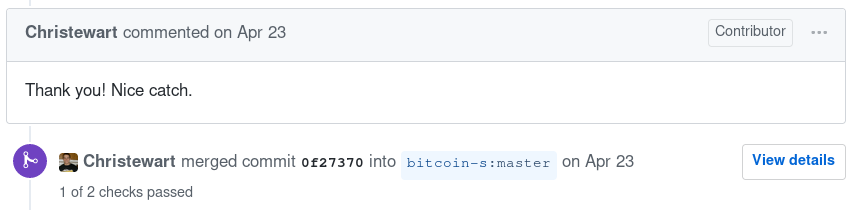
\includegraphics[scale=0.5]{images/bitcoin-s-pr-comment.png}
	\caption{Nice catch comment on our PR \#435 on GitHub}
	\label{fig:output1}
\end{figure}

Here the relevant code of checkTransaction again:
\begin{lstlisting}[language=scala]
  val prevOutputTxIds = transaction.inputs.map(_.previousOutput.txId)
  val noDuplicateInputs = prevOutputTxIds.distinct.size == prevOutputTxIds.size
\end{lstlisting}

What happens, if a TransactionOutPoint (previousOutput) references the same Transaction ID (txId) another does?

According to the Bitcoin protocol this is possible.
A transaction can have multiple outputs that should be referenceable by the next transaction.
What should not be possible is a transaction referencing the same output twice.
This was a bug in Bitcoin Core known as CVE-2018–17144 which was patched on September 18, 2018. \cite{cve201817144}

Here, Bitcoin-S did a bit too much and marked all transaction as invalid, if they referenced a transaction twice in the next transaction.
The fix is, to check on TransactionOutPoint instead of TransactionOutPoint.txId, because TransactionOutPoint contains the txId as well as the output index it references.
\begin{lstlisting}[language=scala]
  val prevOutputs = transaction.inputs.map(_.previousOutput)
  val noDuplicateInputs = prevOutputs.distinct.size == prevOutputs.size
\end{lstlisting}

Since TransactionOutPoint is a case class and Scala has a built in == for case classes there is no need to implement TransactionOutPoint.==.
\begin{figure}[H]
	\centering
		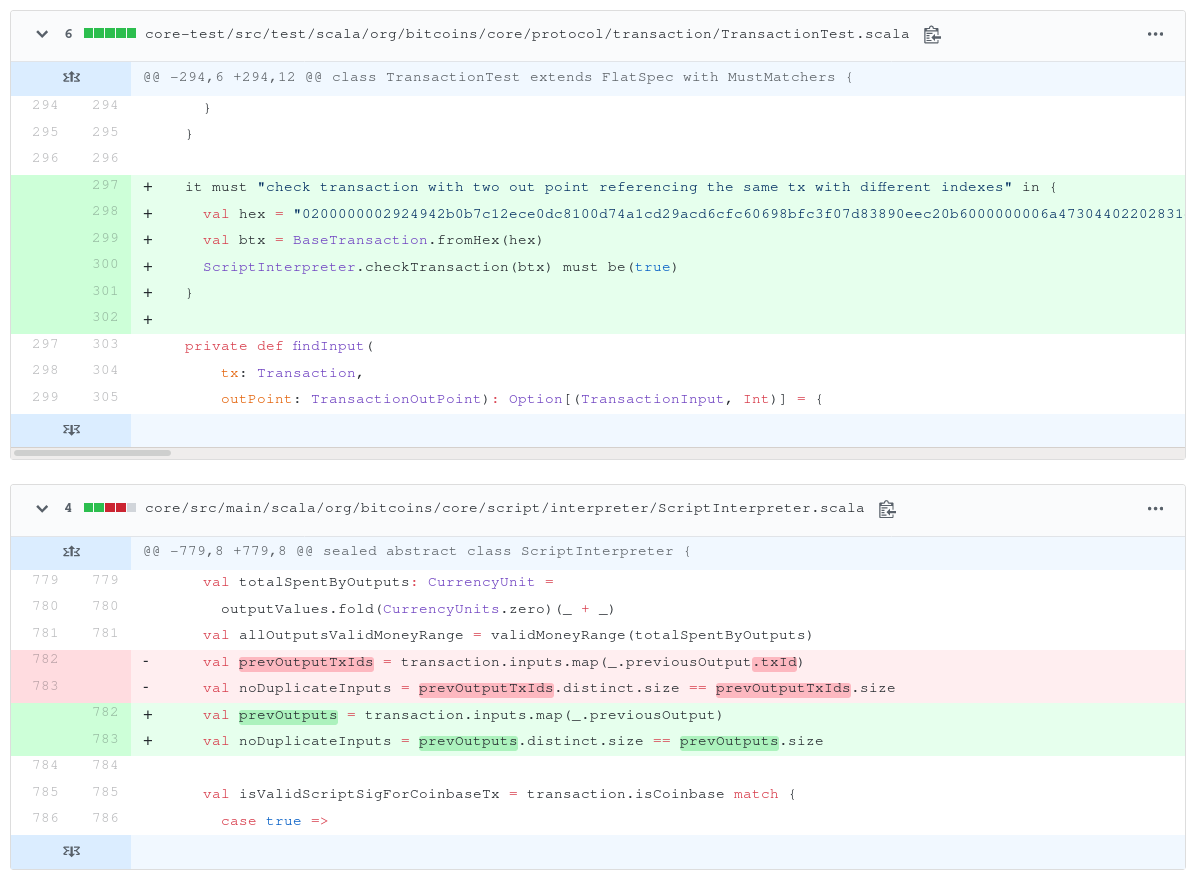
\includegraphics[scale=0.396]{images/bitcoin-s-pr.png}
	\caption{Line changes for PR \#435 from GitHub}
	\label{fig:output1}
\end{figure}

This was fixed in pull request \mypound435 on GitHub\footnote{https://github.com/bitcoin-s/bitcoin-s/pull/435} at April 23, 2019 by us along a unit test to prevent this bug from appearing again in the future.


\section{Adjusting Property}

Trying to integrate Stainless in Bitcoin-S caused a lot of troubles, because of version conflicts.
If you are interested in it you can read more in the appendix \ref{chap:appendix_arb}.

It takes too much time to do it and after some discussion, we decided to extract only the parts of the code that are needed for checkTransaction.

The extracted code has more than 1500 lines.
After running Stainless on it, it throws a really huge bunch of errors about what Stainless can not reason about.
And after fixing some of those errors there appear new ones as we can see in the next chapter.
This would require to change nearly everything of the extracted code.

We arrived at the decision that we need a smaller part to verify.
We have chosen to verify the addition with zero of Bitcoin-Ss CurrencyUnit class as described in the next chapter.
